\documentclass[12pt]{article}
\usepackage[utf8]{inputenc}
\usepackage{amsmath}
\usepackage{multicol}
\usepackage{graphicx}
\usepackage{float}
\usepackage{dsfont}
\usepackage{textcomp}
\usepackage{amsfonts}
\usepackage{hyperref}
\usepackage{amsmath}
\usepackage{csquotes}
%\usepackage[style=authoryear,backend=biber]{biblatex}
%\addbibresource{/mybib.bib}
\hypersetup{
    colorlinks,
    citecolor=black,
    filecolor=black,
    linkcolor=black,
    urlcolor=black
}
\usepackage{cleveref}
\usepackage{fancyhdr}
\setlength{\headheight}{14.5pt}
\renewcommand{\sectionmark}[1]{\markright{#1}{}}
\usepackage[T1]{fontenc}
\usepackage[colorinlistoftodos]{todonotes}
\usepackage[margin=2cm,a4paper]{geometry}
\newgeometry{left=2.0cm,right=2.0cm,top=2.5cm,bottom=2.5cm}
\usepackage{listings}
\setlength{\marginparwidth}{2cm}
\setlength{\parindent}{0pt}
\newcommand{\deriv}{\mathrm{d}}
\title{}
\pagestyle{fancy}
\fancyhf{}
\rhead{Section \thesection}
\lhead{Assignment 2: Astrometry}
\lfoot{PH512: Data Analysis Techniques in Astronomy and Planetary Science}
\rfoot{Page \thepage}
\renewcommand{\headrulewidth}{1pt}
\renewcommand{\footrulewidth}{1pt}
\begin{document}
\begin{titlepage}
\newgeometry{left=1.0in,right=1.0in,top=0.8in,bottom=0.8in}
\newcommand{\HRule}{\rule{\linewidth}{0.5mm}}
\begin{centering} 

%---------------------------------------------------------------------------
%	TITLE SECTION
%---------------------------------------------------------------------------

\includegraphics[scale=0.7]{Images/Uni_of_Kent.png}\\[0.3cm]
\HRule \\ [0.3cm]
\Huge{\bfseries{Astrometry}} \\
\textsc{\large Data Analysis Techniques in Astronomy and Planetary Science}\\ [-0.1cm]
\textsc{\large BSc(Hons) Astronomy, Space Science and Astrophysics}\\ [-0.2cm]
\HRule \\[0.5cm]
%---------------------------------------------------------------------------
\begin{minipage}{0.625\textwidth}
\begin{center} \large
{\large Author: Lukasz R Tomaszewski (lrgt2)} \\[0.2cm]
{\large Date: $29^{th}$ Jan - $12^{th}$ Feb 2020}\\[0.2cm]
{\large PH512 Assignment 2} \\[0.2cm]
{\large Word Count: 1316} \\
\end{center}
\end{minipage}\\[1cm]
\end{centering} 
\begin{tableofcontents}
\end{tableofcontents}
\end{titlepage}
\newpage
%---------------------------------------------------------------------------
%	SECTION 1
%---------------------------------------------------------------------------
\section{Astrometry Analysis}
\label{Section 1}

Astrometry is the measurement of positions, movements and behaviour of celestial bodies but astrometry encounters problems such as; precession, nutation, proper motion, atmospheric refraction and parallax. (\cite{ImageProcessingDilemma}). \\

\begin{figure}[H]
\centering
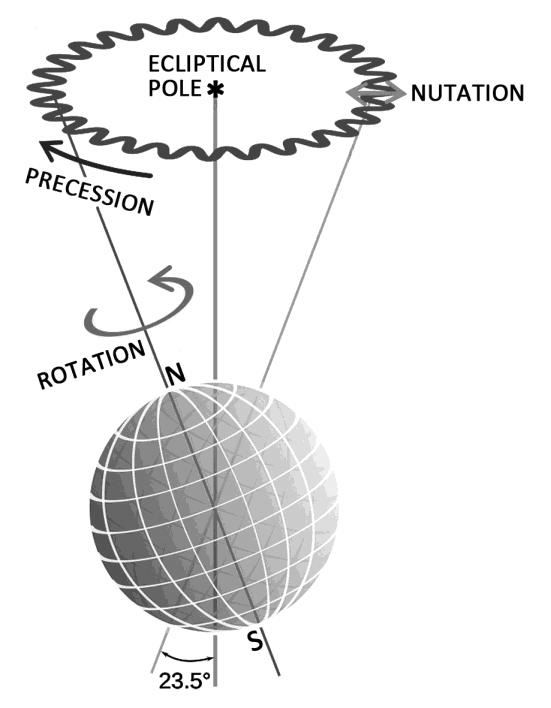
\includegraphics[scale=0.3]{Images/S1/2.png}
\caption{Diagram showing the rotation, precession and nutation of Earth (\cite{RPN}).}
\label{nutation}
\end{figure}

The nutation and precession of a star/ celestial body that moves on its own axis is that its not only rotating but spinning and wobbling alongside its rotation. \cref{nutation} depicts these effects where precession is strongly related to the rotation and nutation is effected but its precession, this can cause reading errors as the nutation and precession vary in time and therefore requires multiple measurements to improve accuracy. The proper motion of a celestial body/ star is that of its true velocity where, the problem arises where to the naked eye, celestial bodies do not appear to have any motion, telescopes eliminate this for closer celestial bodies but when reading at a greater distance the naked eye problem arises again thus requiring multiple measurements over a vast time frame to deuce a celestial bodies proper motion. \\

\begin{figure}[H]
\centering
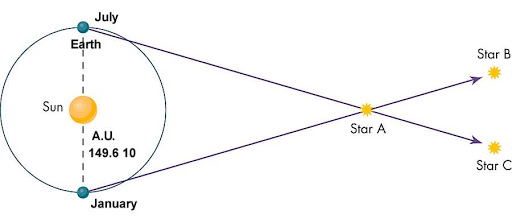
\includegraphics[scale=0.6]{Images/S1/parallax.png}
\caption{Diagram showing the parallax and determining distances to stars (\cite{parallax}).}
\label{parallax}
\end{figure}

The parallax is a measurement used to determine the distance to a celestial body as depicted in \cref{parallax} but as the Earth orbits the Sun, the parallax angle varies and atmospheric refraction from the sun interferes with the ability to make accurate readings and determine the celestial bodies magnitude. Atmospheric refraction is the biggest dilemma as ground based telescopes have to penetrate the Earth's atmosphere that's filled with air that is at different density's and light reflection coming off the sun. With space based telescopes the only atmospheric refraction is that of nearby stars that emit light. 

%---------------------------------------------------------------------------
%	SECTION 2
%---------------------------------------------------------------------------
\section{Astrometry Method}
\label{Section 2}
%---------------------------------------------------------------------------
%	SECTION 2A
%---------------------------------------------------------------------------
\subsection{AIP4WIN Tutorial}
\label{Subsection 2a}

Following the 'AIP4WIN' tutorial (\cite{ImageProcessingTutorial}), three asteroids were located via the analysis of two images of the same cluster of celestial bodies, where image 2 was taken at a later time to image 1. When the images were loaded into the 'AIP4WIN' software it was required to adjust the black/ white contrast ratio from B=307.427 and W=531.430 to: image 1=(B=364.808,W=569.843) and image 2=(B=383.227,W=566.843). This darkens the black empty space background and brightens the white celestial bodies in the foreground/ background so they can be seen easily 

as follows.

\begin{figure}[H]
\begin{multicols}{2}
\centering
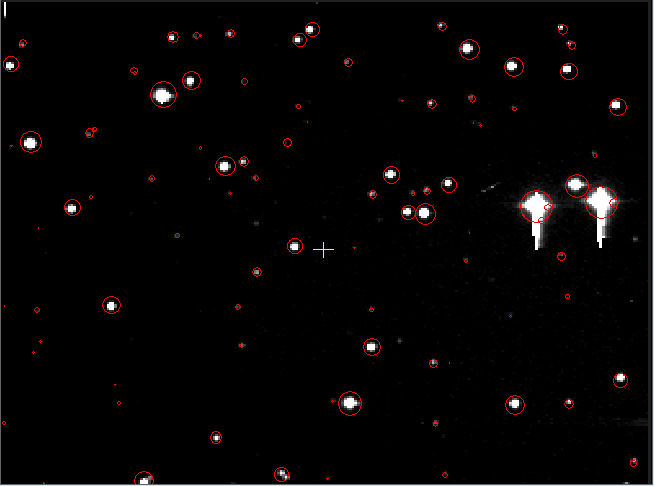
\includegraphics[scale=0.5]{Images/S2/dcdoverlay.PNG}
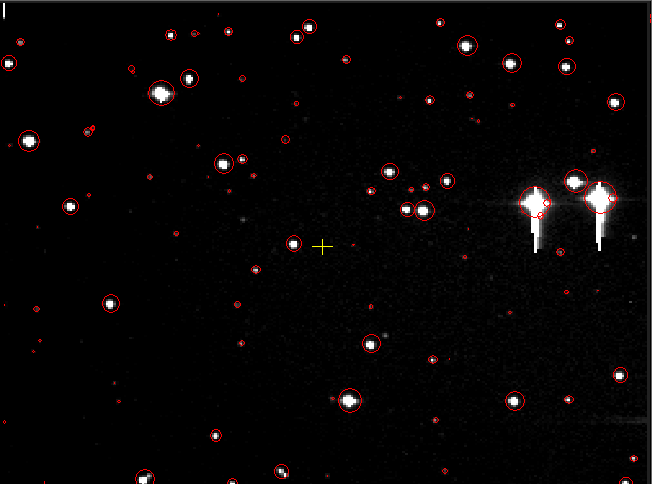
\includegraphics[scale=0.5]{Images/S2/dadoverlay.PNG}
\end{multicols}
\caption{AIP4WIN image of a star cluster with a database overlay.}
\label{Image Overlays}
\end{figure}

The use of the 'blink' tool allows both images to be played at a one second interval, showing one image at a time, thus allowing for movement of celestial bodies to be visual seen. Using this tool, 3 asteroids were found to have moved significantly from the previous image thus are our target objects. Opening the 'Astrometry' tool, image calibration is needed to align the database overlay with the celestial bodies, this was corrected by rotating the image 1 by  +2.6\textdegree and image 2 by +3.0\textdegree and maneuvered over the celestial bodies within each image as seen in \cref{Image Overlays}. The database overlay consists of already surveyed and confirmed celestial bodies and stars to which their positions have been measured, this allows for multiple reference points to be taken as their positions are already known. \\

\begin{table}[H]
\begin{center}
 \footnotesize
 \begin{tabular}{|c||c|c|c||c|c|c||c|c|}
 \hline
 \multicolumn{9}{|c|}{Reference points for both images} \\
 \hline \hline
 Reference & \multicolumn{3}{|c||}{Right Ascension} & \multicolumn{3}{|c||}{Declination} & Pixels$_x$ & Pixels$_y$ \\
 \hline 
 Object& Hrs & Min & Sec & Deg\textdegree & Min & Sec & x-axis & y-axis\\
 \hline \hline
 R1 & 04 & 00 & 12.023 & +21 & 22 & 17.82 & 113.274 & 120.246 \\
 \hline
 R2 & 04 & 00 & 17.219 & +21 & 18 & 33.33 & 134.797 & 198.565 \\
 \hline
 R3 & 04 & 00 & 27.641 & +21 & 22 & 39.45 & 086.157 & 080.320 \\
 \hline
 R4 & 04 & 00 & 32.673 & +21 & 23 & 52.10 & 061.879 & 045.401 \\
 \hline
 R5 & 04 & 00 & 14.956 & +21 & 22 & 39.27 & 150.521 & 084.226 \\
 \hline
 \end{tabular} \\ 
 \caption{Reference points for both images}
 \label{Reference points for both images}
\end{center}
\end{table}

The five reference stars were chosen around the suspected asteroids as seen in \cref{Reference}, all with various visual magnitudes and sizes, the importance of a reference star is that its positions changes infinitesimally on the celestial sphere so that astronomers can track target objects. Each reference points/ stars position on the celestial sphere can be exported to the 'AIP4WIN' data log as seen in \cref{Reference points for both images}, the positions units are labelled in Right Acsension = hours, minutes and seconds whereas the Declination = degrees, arcminutes and arcseconds, these are the standard units for the celestial sphere. 

\begin{figure}[H]
\begin{multicols}{2}
\centering
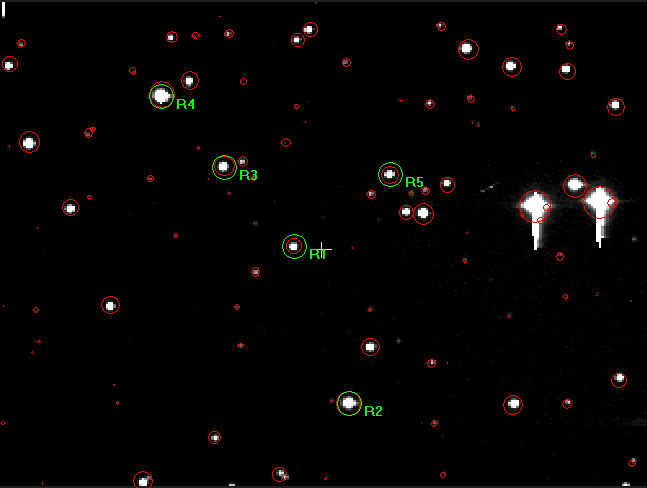
\includegraphics[scale=0.5]{Images/S2/dcdreference.PNG}
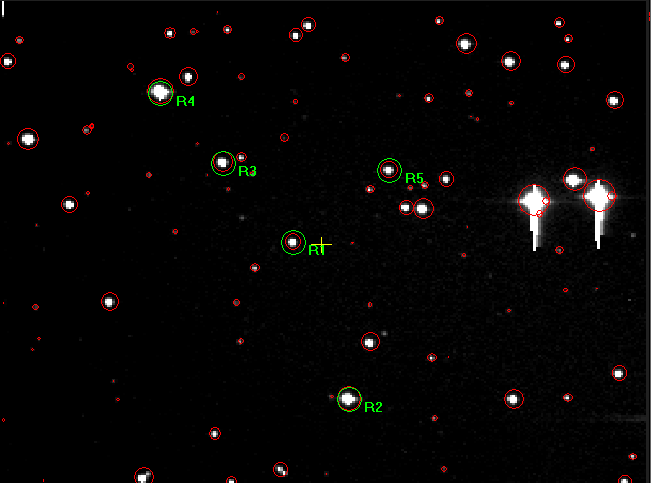
\includegraphics[scale=0.5]{Images/S2/dadreference.PNG}
\end{multicols}
\caption{AIP4WIN second later image of a star cluster with a database overlay and five highlighted reference stars.}
\label{Reference}
\end{figure}


\begin{table}[H]
\begin{center}
 \footnotesize
 \begin{tabular}{|c||c|c|c||c|c|c||c|c||c|}
 \hline
 \multicolumn{10}{|c|}{Target points position before image capture} \\
 \hline \hline
 Target & \multicolumn{3}{|c||}{Right Ascension} & \multicolumn{3}{|c||}{Declination} & Pixels$_x$ & Pixels$_y$ & Magnitude \\
 \hline 
 Object& Hrs & Min & Sec & Deg\textdegree & Min & Sec & x-axis & y-axis & mag\\
 \hline \hline
 Ah102-T1 & 04 & 00 & 13.684 & +21 & 19 & 42.49 & 153.901 & 168.601 & 18.39 \\
 \hline
 Ah102-T2 & 04 & 00 & 22.153 & +21 & 23 & 47.96 & 115.261 & 051.487 & 18.12 \\
 \hline
 Ah102-T3 & 04 & 00 & 25.038 & +21 & 21 & 40.63 & 098.376 & 110.197 & 18.10 \\
 \hline 
 \multicolumn{1}{c}{} \\
 \hline 
 \multicolumn{10}{|c|}{Target points position after image capture} \\
 \hline \hline
 Target & \multicolumn{3}{|c||}{Right Ascension} & \multicolumn{3}{|c||}{Declination} & Pixels$_x$ & Pixels$_y$ & Magnitude\\
 \hline 
 Object& Hrs & Min & Sec & Deg\textdegree & Min & Sec & x-axis & y-axis & mag \\
 \hline \hline
 Ah102-T1 & 04 & 00 & 14.721 & +21 & 19 & 44.77 & 148.716 & 165.793 & 16.35 \\
 \hline
 Ah102-T2 & 04 & 00 & 22.380 & +21 & 23 & 51.23 & 114.096 & 048.486 & 17.82 \\
 \hline
 Ah102-T3 & 04 & 00 & 25.954 & +21 & 21 & 42.29 & 093.731 & 107.747 & 17.85 \\
 \hline 
 \end{tabular} \\ 
 \caption{Target points for both images}
 \label{Target points for both images}
\end{center}
\end{table}

Using the positions of the suspected asteroids from using the 'blink' tool, the target areas are selected in relation to the reference stars as shown in \cref{Target} and their positions on the celestial sphere indicated in \cref{Target points for both images}. The 'blink' tool allows for a clear separation of the asteroids and stars, as the stars motion is very small over a small time in which both of these images were taken, so the stars appear to remain still whereas the asteroids and other fast moving celestial objects appear to have a high velocity so this tool allows for target areas to be created. The target stars: 'Ah102-T1' \& 'Ah102-T3' can be visually seen to be moving in \cref{Target} as they appear at different location in the images, this can be confirmed as \cref{Target points for both images} shows small differences in declination. As this region of space has already been observed, the target stars can be compared to a survey. \\


\begin{figure}[H]
\begin{multicols}{2}
\centering
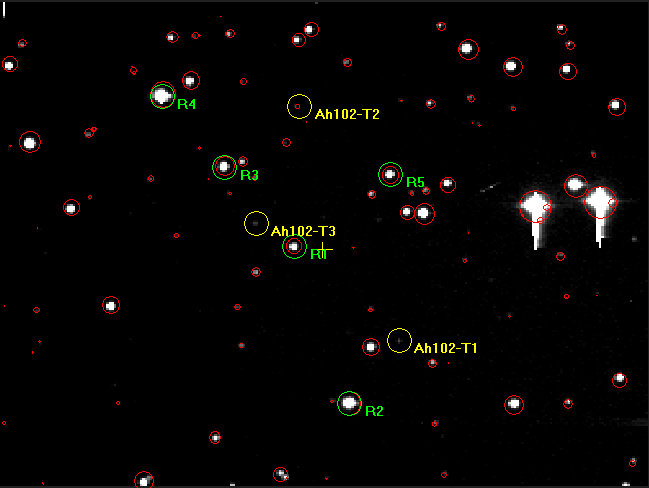
\includegraphics[scale=0.5]{Images/S2/dcdtarget.PNG}
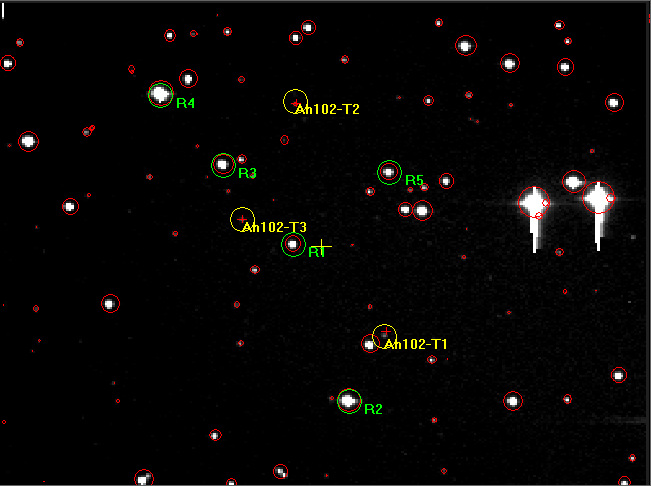
\includegraphics[scale=0.5]{Images/S2/dadtarget.PNG}
\end{multicols}
\caption{AIP4WIN both images of a star cluster with a database overlay and five highlighted reference stars and the three highlighted target asteroids.}
\label{Target}
\end{figure}

\begin{figure}[H]
\centering
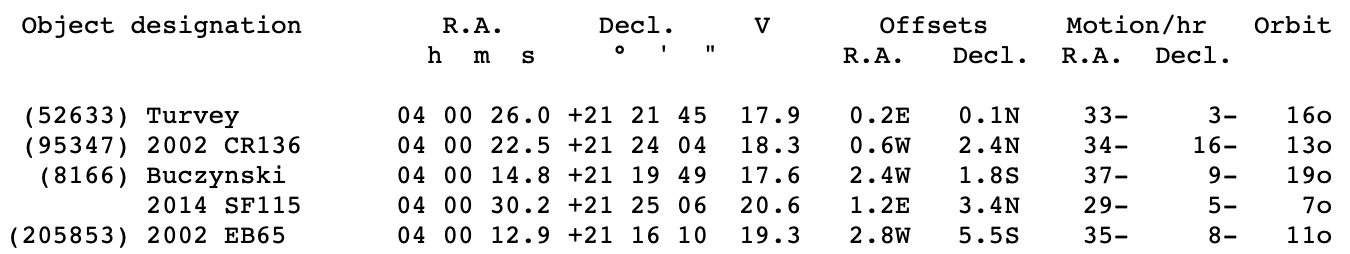
\includegraphics[scale=0.7]{Images/S2/Minor.png}
\caption{Three asteroids in the via the minor planet center. (\cite{Minor})}
\label{Minor planet center}
\end{figure}

Utilizing the Minor Planet Center's survey, the target asteroids positions can be confirmed by comparing \cref{Target points for both images} with \cref{Minor planet center} and each asteroid found in the both images can be deduced as; 
\begin{itemize}
    \item Ah102-T1 = (8166) Buczynski
    \item Ah102-T2 = (95633) 2002 CR136
    \item Ah102-T3 = (52633) Turvey
\end{itemize}

%---------------------------------------------------------------------------
%	SECTION 2B
%---------------------------------------------------------------------------
\subsection{Error Anlaysis}
\label{Subsection 2b}

The error analysis is fairly simple, by exporting the data files from the 'Astrometry' tool on the AIP4WIN software, the error in arcseconds is given for both the right acsension and the declination of the reference stars of both images, to create an error margin for the target objects, the standard deviation equation is used for these errors; \\

\begin{equation}
\sigma = \sqrt{\dfrac{\sum (P_i - P_m)^2}{n-1}}
\end{equation}
Where this equation is used twice per image to decipher the standard deviation of the right ascension and declination. 
\begin{itemize}
    \item n = Number of values for the reference objects, in this case it was 5 for five reference objects
    \item P$_m$ = Mean value for the reference objects right ascension/ declination
    \item P$_i$ = Each reference objects right ascension/ declination 
\end{itemize}

The calculated standard deviation shown in \cref{Error Analysis} can be used to compare the position of the target objects in \cref{Target points for both images} and \cref{Minor planet center}, as declination is in degrees, arc minutes and arcseconds with the position variance in arcseconds, the variance only fits one target object, therefore a misalignment of the database overlay before selecting the reference and target stars is to blame as the overlay would give incorrect values for the right ascension, declination and the errors in arcseconds. 

\begin{table}[H]
\begin{center}
 \footnotesize
 \begin{tabular}{|c||c|c|c||c|c|c|}
 \hline 
 \multicolumn{7}{|c|}{Error analysis of the first Image} \\
 \hline 
 Reference & \multicolumn{3}{|c||}{Right Ascension} & \multicolumn{3}{|c|}{Declination} \\
 \hline 
  Object & Error (") & Std Dev (") & RMS & Error (") & Std Dev (") & RMS \\
 \hline \hline
 R1 & -0.048 & 0.028 & 0.043 & 0.090 & 0.349 & 0.147 \\
 \hline
 R2 & 0.021 & 0.028 & 0.043 & -0.149 & 0.349 & 0.147 \\
 \hline
 R3 & 0.000 & 0.028 & 0.043 & 0.538 & 0.349 & 0.147 \\
 \hline
 R4 & 0.017 & 0.028 & 0.043 & -0.402 & 0.349 & 0.147 \\
 \hline
 R5 & 0.011 & 0.028 & 0.043 & -0.077 & 0.349 & 0.147 \\
 \hline
 \noalign{\vskip 0.5cm} 
 \hline
 \multicolumn{7}{|c|}{Error analysis of the second Image} \\
 \hline 
 Reference & \multicolumn{3}{|c||}{Right Ascension} & \multicolumn{3}{|c|}{Declination} \\
 \hline 
  Object & Error (") & Std Dev (") & RMS & Error (") & Std Dev (") & RMS \\
 \hline \hline
 R1 & -0.195 & 0.116 & 0.068 & -0.039 & 0.220 & 0.014 \\
 \hline
 R2 & 0.087 & 0.116 & 0.068 & 0.070 & 0.220 & 0.014 \\
 \hline
 R3 & -0.012 & 0.116 & 0.068 & 0.362 & 0.220 & 0.014 \\
 \hline
 R4 & 0.076 & 0.116 & 0.068 & -0.236 & 0.220 & 0.014 \\
 \hline
 R5 & 0.045 & 0.116 & 0.068 & -0.030 & 0.220 & 0.014 \\
 \hline
 \end{tabular} \\ 
 \caption{Error analysis of the reference points for both images}
 \label{Error Analysis}
\end{center}
\end{table}

%---------------------------------------------------------------------------
%	SECTION 3
%---------------------------------------------------------------------------
\section{The GAIA Mission}
\label{Section 3}

The GAIA mission's objective is to create a census map the milky way galaxy by observing and surveying millions of stars and celestial bodies, by charting the positions, distance, movements and brightness levels while also discovering an estimated hundreds of thousands new celestial bodies such as quasars and exoplanets and thus creating a three dimensional map of the galaxy. The GAIA spacecraft spans 10m across and consists of two optical telescopes with a camera formed of 106 CCDs with almost one billion pixels that covers a 0.45 field of view that that utilises astrometry, photometry and spectrometry to observe the celestial bodies while the spacecraft rotates at a rate of 60 arcseconds/seconds (\cite{GAIA}). \\ 

While observing millions of stars, a side mission of the GAIA mission is to provide new insight of the theory of relativity, in terms of astrometry it will provide precision improvement on $\lambda$ and the $\beta$ constants as multiple measurements are taken (\cite{General}). This will ultimately improve astronomers understanding of the contents and structure of the milky way galaxy, this will ultimately answer questions such as how the galaxy was formed and more crucially how the universe was created (\cite{over}). \\

\begin{figure}[H]
\centering
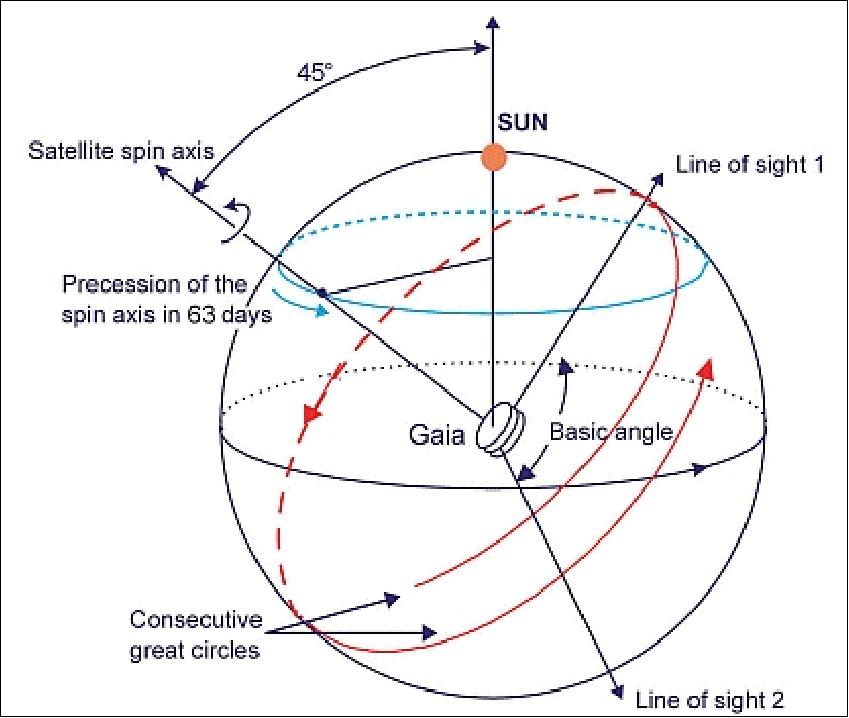
\includegraphics[scale=0.4]{Images/S3/Gaia.jpg}
\caption{Diagram showing how the GAIA spacecraft scans space in relation to the celestial sphere. (\cite{gaiaimage})}
\label{gaia image}
\end{figure}

The GAIA spacecraft will rotate, allowing the two optical telescopes and other instruments to observe celestial object on the celestial sphere, the diagram in \cref{gaia image} shows that the GAIA spacecraft not only rotates but undergoes precession as well \cref{Section 1}. In terms of astrometry, the Gaia spacecraft uses two optical telescopes that measures distances to stars using the parallax to a distance of 10 kPc as an accuracy of 20 micro arcseconds. Over time GAIA is expected to measure the same star/ celestial bodies over 70 times throughout its lifespan, each measurement will be used to discover the proper motion (true velocity) of each star/ celestial body as the proper motion of a star takes years and multiple measurements to deduce its proper motion and to crucially to understand the various star systems mechanics. 

\begin{figure}[H]
\centering
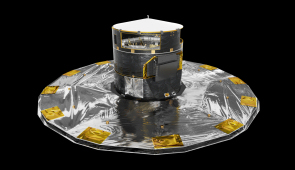
\includegraphics[scale=0.8]{Images/S3/Spacecraft.jpg}
\caption{The GAIA Spacecraft. (\cite{over})}
\label{spacecraft}
\end{figure}

%---------------------------------------------------------------------------
\newpage
\addcontentsline{toc}{section}{References}
%\printbibliography
\bibliographystyle{plain}
\bibliography{mybib.bib}
\end{document}